\documentclass[aspectratio=169]{beamer}
\usepackage{lmodern}
%\usetheme{Madrid}
%\usecolortheme{giantoak}
\newcommand*\oldmacro{}
\let\oldmacro\insertshorttitle
\renewcommand*\insertshorttitle{\oldmacro\hfill\insertframenumber\,/\,\inserttotalframenumber}
\usepackage[framemethod=tikz]{mdframed}

%\usepackage{beamerthemesplit}
\usepackage{textpos}
\usepackage{pgf}
%\logo{\pgfputat{\pgfxy(0,-.4)}{\pgfbox[right,base]{\includegraphics[height=1.0cm]{logo.jpg}}}}
%\newcommand{\nologo}{\setbeamertemplate{logo}{}}
\usepackage{booktabs}
\usepackage{graphicx}
\theoremstyle{principle}
\newtheorem*{principle}{Design Principle}


\titlegraphic{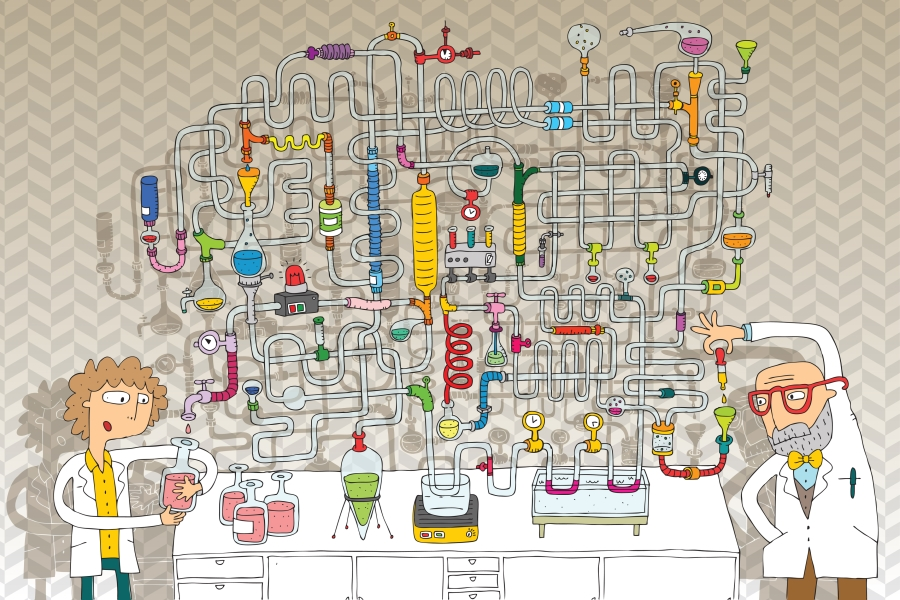
\includegraphics[width=1.0\paperwidth]{causality.jpg}}

\title{Causality}
%\author[Jeremy Kedziora]{Wind Data Science Team\\
%\small{Uptake}}
\date{}

\begin{document}

%{
%%\nologo
%\begin{frame}
%    \maketitle
%\end{frame}
%}
%pages 1-7, 8-9, 14-15.


{
%  \usebackgroundtemplate{
\includegraphics[width=1.0\paperwidth]{statistics-review.jpg}}
  \usebackgroundtemplate{
  %\begin{center}
  	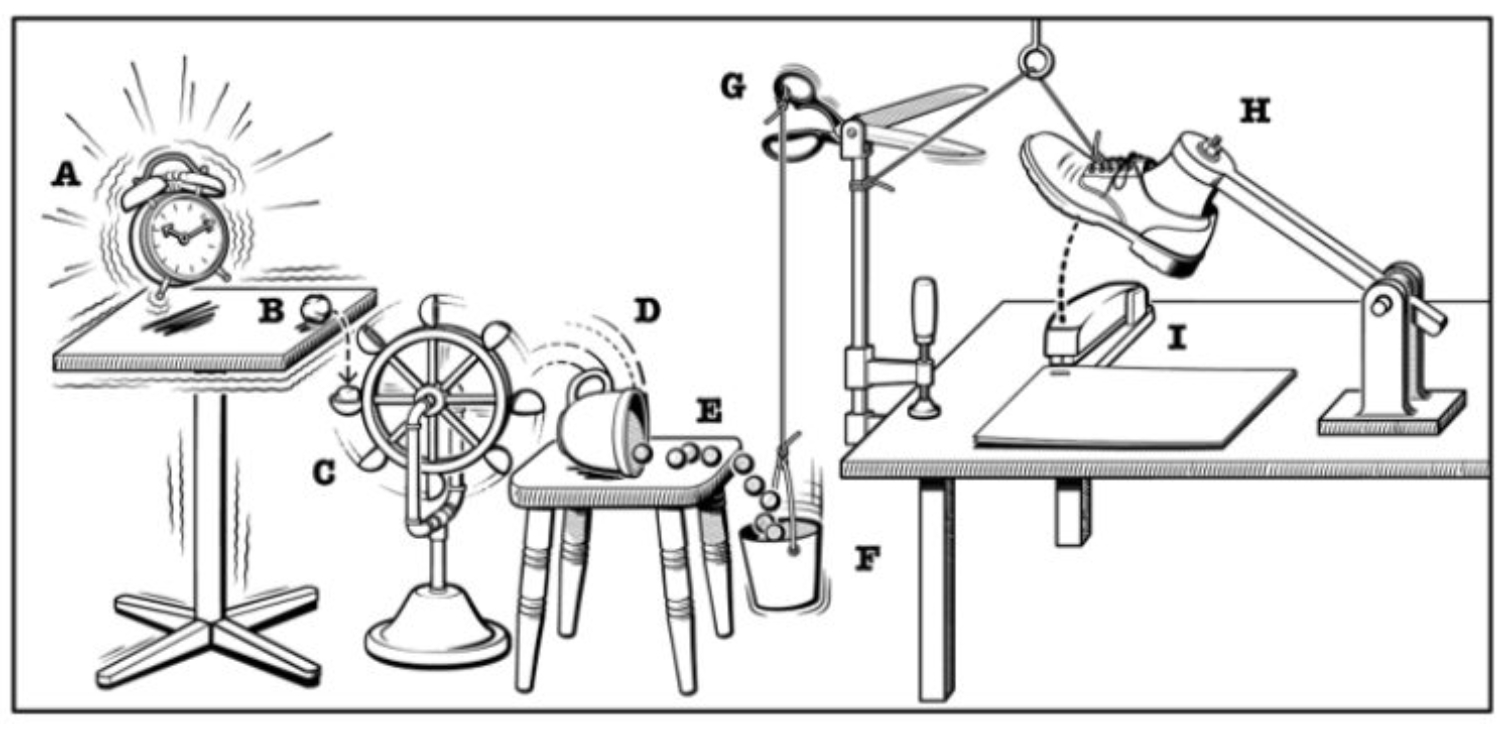
\includegraphics[scale=0.7]{causality.png}
%	\end{center}
	}
  \begin{frame}[plain]
  
\begin{mdframed}[tikzsetting={draw=white,fill=white,fill opacity=0.6,draw opacity=0.4,
               line width=0pt},backgroundcolor=none,leftmargin=20,
               rightmargin=20,innertopmargin=4pt]
\begin{center}
\Huge \textbf{Causality and Causal Inference}
\end{center}
\end{mdframed}

  \end{frame}
}

%@@@@@@@@@@@@@@@@@@@@@@@@@@@@@@@@@@@@@@@@@@@@@@@@@
\begin{frame}
\frametitle{Today:}
\begin{itemize}
\item Introduce the Rubin Causal Model;
\bigskip
\bigskip

\item Discuss the fundamental problem of causal inference;
\bigskip
\bigskip

\item Use descriptive statistics to get around the fundamental problem of causal inference.
\bigskip
\bigskip

\end{itemize}
\end{frame}


%@@@@@@@@@@@@@@@@@@@@@@@@@@@@@@@@@@@@@@@@@@@@@@@@@
\begin{frame}
\frametitle{What is causality?!}
\begin{itemize}
\item In this class we want to use political numbers appropriately -- often this will look like does variable $X$ cause a change in variable $y$:%are concerned with trying to establish the \textbf{why} -- this is a question about \textbf{causality};
\begin{itemize}
\item Does education level change the gender wage gap?
\item Does incumbency confer an advantage?
\item Do nuclear weapons decrease the chance of conflict?
\item Do social safety nets decrease labor?
\end{itemize}
\bigskip
\bigskip
\item Many, many definitions -- here are two to think about:
\begin{itemize}
\item Counterfactual causality:
\begin{itemize}
\item The difference between worlds -- we'll talk about this;
\item In the version of this we will discuss today causality is deterministic;
\end{itemize}
\item Probabilistic causation:
\begin{itemize}
\item A change in a variable will on average cause a change in another variable;
\item This is probabilistic -- note the `on average' part.
\end{itemize}
\end{itemize}
\end{itemize}
\end{frame}

%%@@@@@@@@@@@@@@@@@@@@@@@@@@@@@@@@@@@@@@@@@@@@@@@@@
%\begin{frame}
%\frametitle{What is causality?!}
%\begin{itemize}
%\item In this class we are concerned with trying to establish the \textbf{why} -- this is a question about \textbf{causality};
%\begin{itemize}
%\item Why is there a gender wage gap?
%\item Why do candidates and incumbents win or lose?
%\item Why are some people rich and some people poor?
%\end{itemize}
%\bigskip
%\bigskip
%\item Many, many definitions -- here are two to think about:
%\begin{itemize}
%\item \textbf{Counterfactual causality:}
%\begin{itemize}
%\item \textbf{Blar;}
%\item \textbf{in the version of this we will discuss today causality is deterministic;}
%\end{itemize}
%\item Probabilistic causation:
%\begin{itemize}
%\item
%\item
%\end{itemize}
%\end{itemize}
%\end{itemize}
%\end{frame}

%@@@@@@@@@@@@@@@@@@@@@@@@@@@@@@@@@@@@@@@@@@@@@@@@@
\begin{frame}
\frametitle{The Rubin Causal Model}

\begin{center}
\href{https://psycnet.apa.org/record/1975-06502-001}{...the \color{blue}\underline{causal effect} \color{black} of one treatment, T, over another, C, for a particular unit is the difference between what would have happened if the unit had been exposed to T and what would have happened if the unit had been exposed to C...}
\end{center}
\end{frame}



%@@@@@@@@@@@@@@@@@@@@@@@@@@@@@@@@@@@@@@@@@@@@@@@@@
\begin{frame}
\frametitle{The Rubin Causal Model}
\begin{itemize}
\item \textbf{Example}: a political campaign is seeking money for its `war chest' and wants to know if going door to door to visit party members will increase contributions;
\bigskip
\item Let's think about a party member -- the campaign wants to know:
\begin{itemize}
\item The \textbf{donation} this person will make \textbf{if they get a visit} from the campaign;
\item The \textbf{donation} this person will make \textbf{if they don't get a visit} from the campaign;
\end{itemize}
\bigskip
\item Some useful terms in the Rubin Causal Model:
\begin{itemize}
\item The party member is a \textbf{unit};
\item The visit is a \textbf{treatment};
\item The group that gets no visit is the \textbf{control};
\item The two possible donations are \textbf{potential outcomes}.
\end{itemize}
\end{itemize}
\end{frame}

%@@@@@@@@@@@@@@@@@@@@@@@@@@@@@@@@@@@@@@@@@@@@@@@@@
\begin{frame}
\frametitle{The Rubin Causal Model}
\huge
\begin{table}
\begin{tabular}{ c | c | c | c}
Unit & $Y_i(\mbox{visit})$ & $Y_i(\mbox{none})$ & \color{white}$Y_i(\mbox{visit}) - Y_i(\mbox{none})$ \\
\hline
\hline
  1 & \$675 & \$150 & \color{white}\$525 \\
  \color{white}2 & \color{white}\$3600 & \color{white}\$2500 & \color{white}\$1100\\
  \color{white}3 & \color{white}\$1900 & \color{white}\$3300 & \color{white}-\$1400\\
  \color{white}4 & \color{white}\$2300 & \color{white}\$1000 & \color{white}\$1300\\
  \color{white}5 & \color{white}\$2600 & \color{white}\$2000 & \color{white}\$600\\
  \color{white}6 & \color{white}\$3000 & \color{white}\$0 & \color{white}\$3000\\
  \color{white}7 & \color{white}\$1950 & \color{white}\$2500 & \color{white}-\$550\\
\hline
\hline
\end{tabular}
\end{table}

\end{frame}

%@@@@@@@@@@@@@@@@@@@@@@@@@@@@@@@@@@@@@@@@@@@@@@@@@
\begin{frame}
\frametitle{The Rubin Causal Model}
\huge
\begin{table}
\begin{tabular}{ c | c | c | c}
Unit & $Y_i(\mbox{visit})$ & $Y_i(\mbox{none})$ & \color{white}$Y_i(\mbox{visit}) - Y_i(\mbox{none})$ \\
\hline
\hline
  1 & \$675 & \$150 & \color{white}\$525 \\
  2 & \$3600 & \$2500 & \color{white}\$1100\\
  3 & \$1900 & \$3300 & \color{white}-\$1400\\
  4 & \$2300 & \$1000 & \color{white}\$1300\\
  5 & \$2600 & \$2000 & \color{white}\$600\\
  6 & \$3000 & \$0 & \color{white}\$3000\\
  7 & \$1950 & \$2500 & \color{white}-\$550\\
\hline
\hline
\end{tabular}
\end{table}

\end{frame}

%@@@@@@@@@@@@@@@@@@@@@@@@@@@@@@@@@@@@@@@@@@@@@@@@@
\begin{frame}
\frametitle{The Rubin Causal Model}
\huge
\begin{table}
\begin{tabular}{ c | c | c | c}
Unit & $Y_i(\mbox{visit})$ & $Y_i(\mbox{none})$ & $Y_i(\mbox{visit}) - Y_i(\mbox{none})$ \\
\hline
\hline
  1 & \$675 & \$150 & \$525 \\
  2 & \$3600 & \$2500 & \$1100\\
  3 & \$1900 & \$3300 & -\$1400\\
  4 & \$2300 & \$1000 & \$1300\\
  5 & \$2600 & \$2000 & \$600\\
  6 & \$3000 & \$0 & \$3000\\
  7 & \$1950 & \$2500 & -\$550\\
\hline
\hline
\end{tabular}
\end{table}

\end{frame}

%@@@@@@@@@@@@@@@@@@@@@@@@@@@@@@@@@@@@@@@@@@@@@@@@@
\begin{frame}
\frametitle{The Rubin Causal Model}
\huge
\begin{table}
\begin{tabular}{ c | c | c | c}
Unit & $Y_i(\mbox{visit})$ & $Y_i(\mbox{none})$ & $Y_i(\mbox{visit}) - Y_i(\mbox{none})$ \\
\hline
\hline
  1 & \$675 & ? & \$525 \\
  2 & \$3600 & ? & \$1100\\
  3 & ? & \$3300 & -\$1400\\
  4 & \$2300 & ? & \$1300\\
  5 & ? & \$2000 & \$600\\
  6 & ? & \$0 & \$3000\\
  7 & \$1950 & ? & -\$550\\
\hline
\hline
\end{tabular}
\end{table}

\end{frame}

%@@@@@@@@@@@@@@@@@@@@@@@@@@@@@@@@@@@@@@@@@@@@@@@@@
\begin{frame}
\frametitle{The Rubin Causal Model}
\huge
\begin{table}
\begin{tabular}{ c | c | c | c}
Unit & $Y_i(\mbox{visit})$ & $Y_i(\mbox{none})$ & $Y_i(\mbox{visit}) - Y_i(\mbox{none})$ \\
\hline
\hline
  1 & \$675 & ? & ? \\
  2 & \$3600 & ? & ? \\
  3 & ? & \$3300 & ? \\
  4 & \$2300 & ? & ? \\
  5 & ? & \$2000 & ? \\
  6 & ? & \$0 & ? \\
  7 & \$1950 & ? & ? \\
\hline
\hline
\end{tabular}
\end{table}

\end{frame}

%@@@@@@@@@@@@@@@@@@@@@@@@@@@@@@@@@@@@@@@@@@@@@@@@@
\begin{frame}

\begin{center}
\Huge The \textbf{fundamental problem of causal inference}: one of the potential outcomes is ALWAYS missing.
\end{center}

\end{frame}

%@@@@@@@@@@@@@@@@@@@@@@@@@@@@@@@@@@@@@@@@@@@@@@@@@
\begin{frame}
\frametitle{Estimating Effects: Graphically via Density Plots}
\begin{itemize}
\item Can't observe unit level casual effects directly;
\end{itemize}
\begin{center}
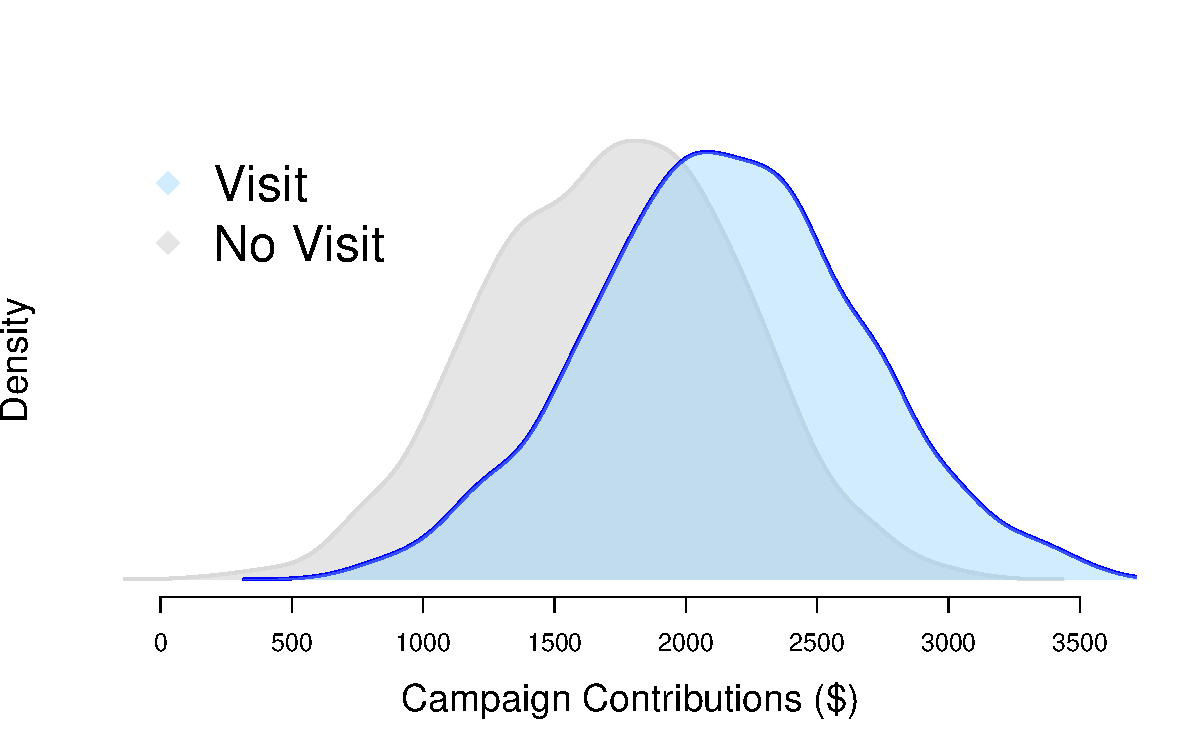
\includegraphics[scale=0.45]{causal_inference.pdf}
\end{center}
\end{frame}

%@@@@@@@@@@@@@@@@@@@@@@@@@@@@@@@@@@@@@@@@@@@@@@@@@
\begin{frame}
\frametitle{Estimating Effects: Average Causal Effect}
\begin{itemize}
\item Can't observe unit level casual effects directly;
\bigskip
\bigskip
\item Can compute an average causal effect -- for $n_T$ units in the treatment group and $n_C$ units in the control group:
\begin{align*}
\frac{1}{n_T}\sum_iY_i(\mbox{T}) - \frac{1}{n_C}\sum_iY_i(\mbox{C});
\end{align*}
\bigskip
\item For our example:
\begin{align*}
\frac{\$675 + \$3600 + \$2300 + \$1950}{4} - \frac{\$3300 + \$2000 + \$0}{3} \approx \$365.
\end{align*}
\end{itemize}
\end{frame}

%@@@@@@@@@@@@@@@@@@@@@@@@@@@@@@@@@@@@@@@@@@@@@@@@@
\begin{frame}
\frametitle{Estimating Effects: Average Causal Effect}
\begin{itemize}
\item Can't observe unit level casual effects directly;
\bigskip
\bigskip
\item Can compute an average causal effect -- for $n_T$ party members in the visit group and $n_C$ party members in the no visit group:
\begin{align*}
\frac{1}{n_T}\sum_iY_i(\mbox{visit}) - \frac{1}{n_C}\sum_iY_i(\mbox{none});
\end{align*}
\bigskip
\item For our example:
\begin{align*}
\frac{\$675 + \$3600 + \$2300 + \$1950}{4} - \frac{\$3300 + \$2000 + \$0}{3} \approx \$365.
\end{align*}
\end{itemize}
\end{frame}

%@@@@@@@@@@@@@@@@@@@@@@@@@@@@@@@@@@@@@@@@@@@@@@@@@
\begin{frame}
\frametitle{Estimating Effects: Inferring Unit Level Outcomes}
\begin{itemize}
\item Can't observe unit level casual effects directly;
\bigskip
\item So what can we do?  We can \textbf{infer} unit level effects by making an assumption -- consider \textbf{a unit in the treatment group}:
\begin{align*}
\underbrace{Y_i(\mbox{T})}_{\mbox{Observed!}} - Y_i(\mbox{C}) &= Y_i^*\\
\color{white}\underbrace{Y_i(\mbox{T})}_{\mbox{Observed!}} - Y_i(\mbox{C}) &\color{white}= \underbrace{\frac{1}{n_T}\sum_iY_i(\mbox{T}) - \frac{1}{n_C}\sum_iY_i(\mbox{C})}_{\mbox{Observed!}}\\
\color{white}Y_i(\mbox{C}) &\color{white}= \underbrace{Y_i(\mbox{T})}_{\mbox{Observed!}} - \underbrace{\left(\frac{1}{n_T}\sum_iY_i(\mbox{T}) - \frac{1}{n_C}\sum_iY_i(\mbox{C})\right)}_{\mbox{Observed!}}
\end{align*}
\item[] \color{white} This is called the \textbf{assumption of constant effect}.
\end{itemize}
\end{frame}

%@@@@@@@@@@@@@@@@@@@@@@@@@@@@@@@@@@@@@@@@@@@@@@@@@
\begin{frame}
\frametitle{Estimating Effects: Inferring Unit Level Outcomes}
\begin{itemize}
\item Can't observe unit level casual effects directly;
\bigskip
\item So what can we do?  We can \textbf{infer} unit level effects by making an assumption -- consider \textbf{a unit in the treatment group}:
\begin{align*}
\underbrace{Y_i(\mbox{T})}_{\mbox{Observed!}} - Y_i(\mbox{C}) &= Y_i^*\\
\underbrace{Y_i(\mbox{T})}_{\mbox{Observed!}} - Y_i(\mbox{C}) &= \underbrace{\frac{1}{n_T}\sum_iY_i(\mbox{T}) - \frac{1}{n_C}\sum_iY_i(\mbox{C})}_{\mbox{Observed!}}\\
Y_i(\mbox{C}) &= \underbrace{Y_i(\mbox{T})}_{\mbox{Observed!}} - \underbrace{\left(\frac{1}{n_T}\sum_iY_i(\mbox{T}) - \frac{1}{n_C}\sum_iY_i(\mbox{C})\right)}_{\mbox{Observed!}}
\end{align*}
\item This is called the \textbf{assumption of constant effect}.
\end{itemize}
\end{frame}

%@@@@@@@@@@@@@@@@@@@@@@@@@@@@@@@@@@@@@@@@@@@@@@@@@
\begin{frame}
\frametitle{Estimating Effects: Inferring Unit Level Outcomes}
\begin{itemize}
\item Can't observe unit level casual effects directly;
\bigskip
\item So what can we do?  We can \textbf{infer} unit level effects by making an assumption -- consider \textbf{a unit in the control group}:
\begin{align*}
Y_i(\mbox{T}) - \underbrace{Y_i(\mbox{C})}_{\mbox{Observed!}} &= Y_i^*\\
Y_i(\mbox{T}) - \underbrace{Y_i(\mbox{C})}_{\mbox{Observed!}} &= \underbrace{\frac{1}{n_T}\sum_iY_i(\mbox{T}) - \frac{1}{n_C}\sum_iY_i(\mbox{C})}_{\mbox{Observed!}}\\
Y_i(\mbox{T}) &= \underbrace{Y_i(\mbox{C})}_{\mbox{Observed!}} + \underbrace{\left(\frac{1}{n_T}\sum_iY_i(\mbox{T}) - \frac{1}{n_C}\sum_iY_i(\mbox{C})\right)}_{\mbox{Observed!}}
\end{align*}
\item This is called the \textbf{assumption of constant effect}.
\end{itemize}
\end{frame}

%@@@@@@@@@@@@@@@@@@@@@@@@@@@@@@@@@@@@@@@@@@@@@@@@@
\begin{frame}
\frametitle{Estimating Effects: Inferring Unit Level Outcomes}
\huge
\begin{table}
\begin{tabular}{ c | c | c | c}
Unit & $Y_i(\mbox{visit})$ & $Y_i(\mbox{none})$ & $Y_i(\mbox{visit}) - Y_i(\mbox{none})$ \\
\hline
\hline
  1 & \$675 & ? & ? \\
  2 & \$3600 & ? & ? \\
  3 & ? & \$3300 & ? \\
  4 & \$2300 & ? & ? \\
  5 & ? & \$2000 & ? \\
  6 & ? & \$0 & ? \\
  7 & \$1950 & ? & ? \\
\hline
\hline
\end{tabular}
\end{table}

\end{frame}

%@@@@@@@@@@@@@@@@@@@@@@@@@@@@@@@@@@@@@@@@@@@@@@@@@
\begin{frame}
\frametitle{Estimating Effects: Inferring Unit Level Outcomes}
\huge
\begin{table}
\begin{tabular}{ c | c | c | c}
Unit & $Y_i(\mbox{visit})$ & $Y_i(\mbox{none})$ & $Y_i(\mbox{visit}) - Y_i(\mbox{none})$ \\
\hline
\hline
  1 & \$675 & ? & \$365 \\
  2 & \$3600 & ? & \$365 \\
  3 & ? & \$3300 & \$365 \\
  4 & \$2300 & ? & \$365 \\
  5 & ? & \$2000 & \$365 \\
  6 & ? & \$0 & \$365 \\
  7 & \$1950 & ? & \$365 \\
\hline
\hline
\end{tabular}
\end{table}

\end{frame}

%@@@@@@@@@@@@@@@@@@@@@@@@@@@@@@@@@@@@@@@@@@@@@@@@@
\begin{frame}
\frametitle{Estimating Effects: Inferring Unit Level Outcomes}
\huge
\begin{table}
\begin{tabular}{ c | c | c | c}
Unit & $Y_i(\mbox{visit})$ & $Y_i(\mbox{none})$ & $Y_i(\mbox{visit}) - Y_i(\mbox{none})$ \\
\hline
\hline
  1 & \$675 & \textbf{\$310} & \$365 \\
  2 & \$3600 & \textbf{\$3235} & \$365 \\
  3 & \textbf{\$3665} & \$3300 & \$365 \\
  4 & \$2300 & \textbf{\$1935} & \$365 \\
  5 & \textbf{\$2365} & \$2000 & \$365 \\
  6 & \textbf{\$365} & \$0 & \$365 \\
  7 & \$1950 & \textbf{\$1585} & \$365 \\
\hline
\hline
\end{tabular}
\end{table}

\end{frame}

%@@@@@@@@@@@@@@@@@@@@@@@@@@@@@@@@@@@@@@@@@@@@@@@@@
\begin{frame}
\frametitle{Assignment Effects}
\begin{itemize}
\item Fair warning 1: the assignment of units to the treatment and the control groups is \textbf{very consequential};
\bigskip
\bigskip
\item Question: how many ways are there to assign our 7 party members?
\begin{align*}
\color{white}\mbox{Answer: }2^7 = 128;
\end{align*}
\bigskip
\item Question: how many ways would there be to assign 1000 party members?
\begin{align*}
\color{white}\mbox{Answer: }2^{1000} = 10^{301}.
\end{align*}
\end{itemize}
\end{frame}

%@@@@@@@@@@@@@@@@@@@@@@@@@@@@@@@@@@@@@@@@@@@@@@@@@
\begin{frame}
\frametitle{Assignment Effects}
\begin{itemize}
\item Fair warning 1: the assignment of units to the treatment and the control groups is \textbf{very consequential};
\bigskip
\bigskip
\item Question: how many ways are there to assign our 7 party members?
\begin{align*}
\mbox{Answer: }2^7 - 2 = 126;
\end{align*}
\bigskip
\item Question: how many ways would there be to assign 1000 party members?
\begin{align*}
\mbox{Answer: }2^{1000} - 2 \approx 10^{301}.
\end{align*}
\end{itemize}
\end{frame}

%@@@@@@@@@@@@@@@@@@@@@@@@@@@@@@@@@@@@@@@@@@@@@@@@@
\begin{frame}
\frametitle{Assignment Effects}
\huge
\begin{table}
\begin{tabular}{ c | c | c | c}
Unit & $Y_i(\mbox{visit})$ & $Y_i(\mbox{none})$ & \color{white}$Y_i(\mbox{visit}) - Y_i(\mbox{none})$ \\
\hline
\hline
  1 & \textbf{\$675} & \color{gray}\$150 & \\
  2 & \textbf{\$3600} & \color{gray}\$2500 & \\
  3 & \color{gray}\$1900 & \textbf{\$3300} &Average CE was: \\
  4 & \textbf{\$2300} & \color{gray}\$1000 & \$365\\
  5 & \color{gray}\$2600 & \textbf{\$2000} & \\
  6 & \color{gray}\$3000 & \textbf{\$0} & \\
  7 & \textbf{\$1950} & \color{gray}\$2500 & \\
\hline
\hline
\end{tabular}
\end{table}

\end{frame}

%@@@@@@@@@@@@@@@@@@@@@@@@@@@@@@@@@@@@@@@@@@@@@@@@@
\begin{frame}
\frametitle{Assignment Effects}
\huge
\begin{table}
\begin{tabular}{ c | c | c | c}
Unit & $Y_i(\mbox{visit})$ & $Y_i(\mbox{none})$ & \color{white}$Y_i(\mbox{visit}) - Y_i(\mbox{none})$ \\
\hline
\hline
  1 & \textbf{\$675} & \color{gray}\$150 & \\
  2 & \color{gray}\$3600 & \textbf{\$2500} & \\
  3 & \color{gray}\$1900 & \textbf{\$3300} &Average CE is: \\
  4 & \color{gray}\$2300 & \textbf{\$1000} & -\$1208\\
  5 & \color{gray}\$2600 & \textbf{\$2000} & \\
  6 & \color{gray}\$3000 & \textbf{\$0} & \\
  7 & \color{gray}\$1950 & \textbf{\$2500} & \\
\hline
\hline
\end{tabular}
\end{table}

\end{frame}

%@@@@@@@@@@@@@@@@@@@@@@@@@@@@@@@@@@@@@@@@@@@@@@@@@
\begin{frame}
\frametitle{Assignment Effects: a perfect campaign manager}
\huge
\begin{table}
\begin{tabular}{ c | c | c | c}
Unit & $Y_i(\mbox{visit})$ & $Y_i(\mbox{none})$ & \color{white}$Y_i(\mbox{visit}) - Y_i(\mbox{none})$ \\
\hline
\hline
  1 & \textbf{\$675} & \color{gray}\$150 & \\
  2 & \textbf{\$3600} & \color{gray}\$2500 & \\
  3 & \color{gray}\$1900 & \textbf{\$3300} &Average CE is: \\
  4 & \textbf{\$2300} & \color{gray}\$1000 & -\$465\\
  5 & \textbf{\$2600} & \color{gray}\$2000 & \\
  6 & \textbf{\$3000} & \color{gray}\$0 & \\
  7 & \color{gray}\$1950 & \textbf{\$2500} & \\
\hline
\hline
\end{tabular}
\end{table}

\end{frame}

%@@@@@@@@@@@@@@@@@@@@@@@@@@@@@@@@@@@@@@@@@@@@@@@@@
\begin{frame}
\frametitle{Assignment Effects: a perfect visit advocate}
\huge
\begin{table}
\begin{tabular}{ c | c | c | c}
Unit & $Y_i(\mbox{visit})$ & $Y_i(\mbox{none})$ & \color{white}$Y_i(\mbox{visit}) - Y_i(\mbox{none})$ \\
\hline
\hline
  1 & \color{gray}\$675 & \textbf{\$150} & \\
  2 & \textbf{\$3600} & \color{gray}\$2500 & \\
  3 & \textbf{\$1900} & \color{gray}\$3300 &Average CE is: \\
  4 & \color{gray}\$2300 & \textbf{\$1000} & \$2129\\
  5 & \textbf{\$2600} & \color{gray}\$2000 & \\
  6 & \color{gray}\$3000 & \textbf{\$0} & \\
  7 & \textbf{\$1950} & \color{gray}\$2500 & \\
\hline
\hline
\end{tabular}
\end{table}

\end{frame}

%@@@@@@@@@@@@@@@@@@@@@@@@@@@@@@@@@@@@@@@@@@@@@@@@@
\begin{frame}
\frametitle{Assignment Effects}
\begin{center}
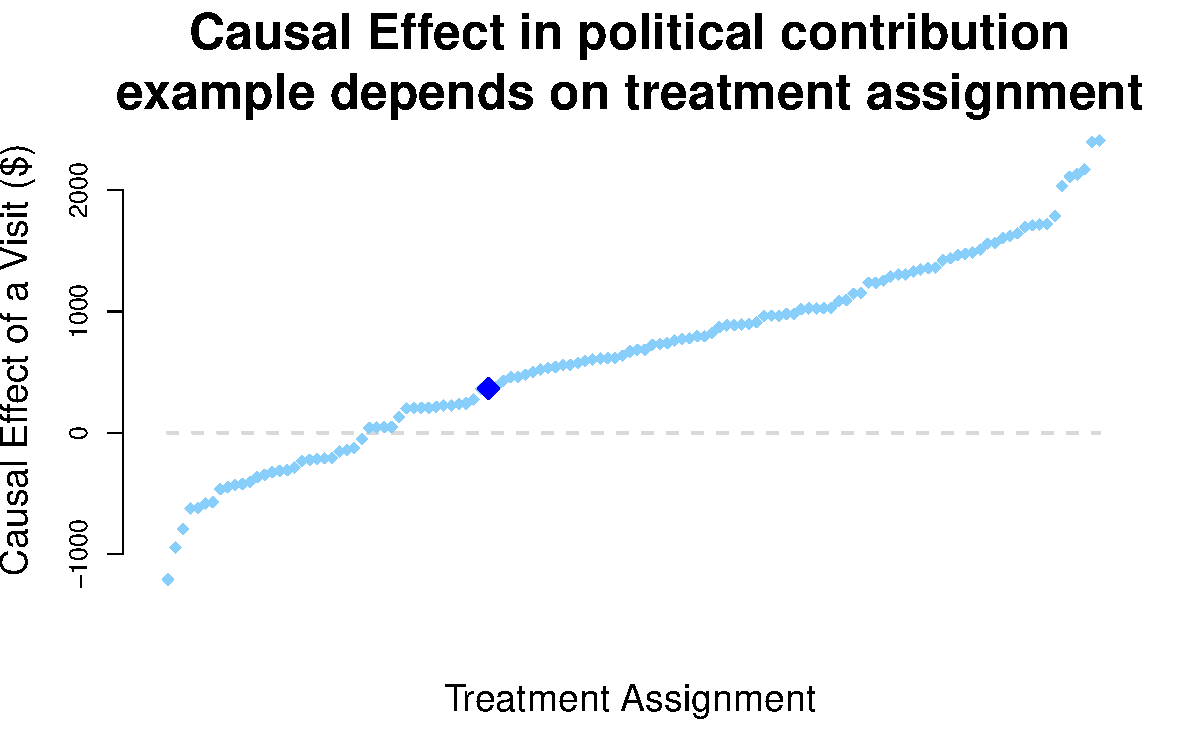
\includegraphics[scale=0.6]{assignment_effects.pdf}
\end{center}
\end{frame}

%%@@@@@@@@@@@@@@@@@@@@@@@@@@@@@@@@@@@@@@@@@@@@@@@@@
%\begin{frame}
%\frametitle{Assignment Effects}
%\begin{itemize}
%\item What is the major issue in the `perfect visit advocate' example?
%\begin{itemize}
%\item[]\color{white} Low contributors are assigned to the control group...
%\item[]\color{white} ...so that contributions are related to assignments;
% \end{itemize}
%\bigskip
%\item How could this happen?  \color{white}Not hard to imagine -- correlate assignment with income:
%\begin{itemize}
%\item[]\color{white} Control group (no visit) entirely composed of lowest 20\% of income distribution;
%\item[]\color{white} Treatment group (visit) entirely composed of highest 20\% of income distribution;
%\end{itemize}
%\bigskip
%\item[]\color{white} How to deal with this?  First steps: large sample, randomized assignment;
%\begin{itemize}
%\item[]\color{white} As sample size increases the probability of an imbalance in some unobserved characteristic between treatment and control gets arbitrarily low;
%\item[]\color{white} Treatment assignment is independent of the potential outcomes.
%\end{itemize}
%\end{itemize}
%\end{frame}
%
%%@@@@@@@@@@@@@@@@@@@@@@@@@@@@@@@@@@@@@@@@@@@@@@@@@
%\begin{frame}
%\frametitle{Assignment Effects}
%\begin{itemize}
%\item What is the major issue in the `perfect visit advocate' example?
%\begin{itemize}
%\item Low contributors are assigned to the control group...
%\item ...so that contributions are related to assignments;
% \end{itemize}
%\bigskip
%\item How could this happen?  \color{white}Not hard to imagine -- correlate assignment with income:
%\begin{itemize}
%\item[]\color{white} Control group (no visit) entirely composed of lowest 20\% of income distribution;
%\item[]\color{white} Treatment group (visit) entirely composed of highest 20\% of income distribution;
%\end{itemize}
%\bigskip
%\item[]\color{white} How to deal with this?  First steps: large sample, randomized assignment;
%\begin{itemize}
%\item[]\color{white} As sample size increases the probability of an imbalance in some unobserved characteristic between treatment and control gets arbitrarily low;
%\item[]\color{white} Treatment assignment is independent of the potential outcomes.
%\end{itemize}
%\end{itemize}
%\end{frame}
%
%%@@@@@@@@@@@@@@@@@@@@@@@@@@@@@@@@@@@@@@@@@@@@@@@@@
%\begin{frame}
%\frametitle{Assignment Effects}
%\begin{itemize}
%\item What is the major issue in the `perfect visit advocate' example?
%\begin{itemize}
%\item Low contributors are assigned to the control group...
%\item ...so that contributions are related to assignments;
% \end{itemize}
%\bigskip
%\item How could this happen?  Not hard to imagine -- correlate assignment with income:
%\begin{itemize}
%\item Control group (no visit) entirely composed of lowest 20\% of income distribution;
%\item Treatment group (visit) entirely composed of highest 20\% of income distribution;
%\end{itemize}
%\bigskip
%\item[]\color{white} How to deal with this?  First steps: large sample, randomized assignment;
%\begin{itemize}
%\item[]\color{white} As sample size increases the probability of an imbalance in some unobserved characteristic between treatment and control gets arbitrarily low;
%\item[]\color{white} Treatment assignment is independent of the potential outcomes.
%\end{itemize}
%\end{itemize}
%\end{frame}
%
%%@@@@@@@@@@@@@@@@@@@@@@@@@@@@@@@@@@@@@@@@@@@@@@@@@
%\begin{frame}
%\frametitle{Assignment Effects}
%\begin{itemize}
%\item What is the major issue in the `perfect visit advocate' example?
%\begin{itemize}
%\item Low contributors are assigned to the control group...
%\item ...so that contributions are related to assignments;
% \end{itemize}
%\bigskip
%\item How could this happen?  Not hard to imagine -- correlate assignment with income:
%\begin{itemize}
%\item Control group (no visit) entirely composed of lowest 20\% of income distribution;
%\item Treatment group (visit) entirely composed of highest 20\% of income distribution;
%\end{itemize}
%\bigskip
%\item How to deal with this?  First steps: \textbf{large sample}, \textbf{randomized assignment};
%\begin{itemize}
%\item As sample size increases the probability of an imbalance in some unobserved characteristic between treatment and control gets arbitrarily low;
%\item Treatment assignment is independent of the potential outcomes.
%\end{itemize}
%\end{itemize}
%\end{frame}
%
%%@@@@@@@@@@@@@@@@@@@@@@@@@@@@@@@@@@@@@@@@@@@@@@@@@
%\begin{frame}
%\frametitle{Stable Unit Treatment Value Assumption}
%\begin{itemize}
%\item We estimated the causal effect in a really simple way in the Rubin Causal Model:% -- the difference in average observed outcome between treatment and control groups:
%\begin{align*}
%\frac{1}{n_T}\sum_iY_i(\mbox{T}) - \frac{1}{n_C}\sum_iY_i(\mbox{C})
%\end{align*}
%\item Fair warning 2: should acknowledge that potential outcomes could depend on other stuff, e.g.:
%\begin{align*}
%Y_1(\hspace{-13.5mm}\underbrace{\mbox{T}}_{\mbox{assignment for unit 1}}\hspace{-13.5mm},\hspace{-5mm}\overbrace{\mbox{T},\mbox{C},\mbox{T},\mbox{C},\mbox{C},\mbox{T}}^{\mbox{assignments for rest}}\hspace{-3mm})
%\end{align*}
%\item[]\color{white} It is a modeling assumption that we can write:
%\begin{align*}
%Y_1(\mbox{T},\mbox{T},\mbox{C},\mbox{T},\mbox{C},\mbox{C},\mbox{T}) = Y_1(T);
%\end{align*}
%This is called the \textbf{Stable Unit Treatment Value Assumption} (SUTVA)!
%\end{itemize}
%\end{frame}
%
%%@@@@@@@@@@@@@@@@@@@@@@@@@@@@@@@@@@@@@@@@@@@@@@@@@
%\begin{frame}
%\frametitle{Stable Unit Treatment Value Assumption}
%\begin{itemize}
%\item We estimated the causal effect in a really simple way in the Rubin Causal Model:% -- the difference in average observed outcome between treatment and control groups:
%\begin{align*}
%\frac{1}{n_T}\sum_iY_i(\mbox{T}) - \frac{1}{n_C}\sum_iY_i(\mbox{C})
%\end{align*}
%\item Fair warning 2: should acknowledge that potential outcomes could depend on other stuff, e.g.:
%\begin{align*}
%Y_1(\hspace{-13.5mm}\underbrace{\mbox{T}}_{\mbox{assignment for unit 1}}\hspace{-13.5mm},\hspace{-5mm}\overbrace{\mbox{T},\mbox{C},\mbox{T},\mbox{C},\mbox{C},\mbox{T}}^{\mbox{assignments for rest}}\hspace{-3mm})
%\end{align*}
%\item It is a modeling assumption that we can write:
%\begin{align*}
%Y_1(\mbox{T},\mbox{T},\mbox{C},\mbox{T},\mbox{C},\mbox{C},\mbox{T}) = Y_1(T);
%\end{align*}
%This is called the \textbf{Stable Unit Treatment Value Assumption} (SUTVA)!
%\end{itemize}
%\end{frame}
%
%%@@@@@@@@@@@@@@@@@@@@@@@@@@@@@@@@@@@@@@@@@@@@@@@@@
%\begin{frame}
%\frametitle{Stable Unit Treatment Value Assumption}
%\begin{itemize}
%\item What does SUTVA mean?  It means:
%\begin{itemize}
%\item Potential outcomes for each unit (party member) are not related to treatment assignment for any other unit;
%\item There are no unmodeled spillover effects of any kind;
%\end{itemize}
%\bigskip
%\item How could this fail to hold?  Imagine that party members 1 and 2 live in the same household!  Then:
%\begin{itemize} 
%\item SUTVA is pretty dubious and...
%\item ...there are four, totally reasonable potential outcomes to think about:
%\end{itemize}
%\end{itemize}
%\Large
%\begin{table}
%\begin{tabular}{ c | c | c | c | c}
%Unit & $Y_i(\mbox{visit,visit})$ & $Y_i(\mbox{visit},\mbox{none})$ & $Y_i(\mbox{none},\mbox{visit})$ & $Y_i(\mbox{none},\mbox{none})$ \\
%\hline
%\hline
%  1 & \$675 & ? & ? & ? \\
%  2 & \vdots & \vdots & \vdots & \vdots \\
%\hline
%\hline
%\end{tabular}
%\end{table}
%
%\end{frame}
%
%%@@@@@@@@@@@@@@@@@@@@@@@@@@@@@@@@@@@@@@@@@@@@@@@@@
%\begin{frame}
%\frametitle{Stable Unit Treatment Value Assumption}
%\begin{itemize}
%\item How many causal effects are there?
%\begin{align*}
%Y_i(\mbox{visit},\mbox{none}) &- Y_i(\mbox{none},\mbox{none}) \hspace{5mm}\mbox{ CE of treatment on 1 given 2 untreated}\\
%Y_i(\mbox{none},\mbox{visit}) &- Y_i(\mbox{none},\mbox{none}) \hspace{5mm}\mbox{ Spillover for a not treated 1 given 2 treated}\\
%Y_i(\mbox{visit,visit}) &- Y_i(\mbox{none},\mbox{visit}) \hspace{6mm}\mbox{ CE of treatment on 1 given 2 treated}\\
%Y_i(\mbox{visit,visit}) &- Y_i(\mbox{visit},\mbox{none}) \hspace{6mm}\mbox{ Spillover for a treated 1 given 2 treated}
%\end{align*}
%
%\item[] \color{white}\href{https://community.lawschool.cornell.edu/wp-content/uploads/2020/12/Green-presentation-on-SUTVA-for-CELS.pdf}{\underline{Spillover examples}} when SUTVA does not hold:
%\begin{itemize}
%\item[] \color{white} \textbf{Contagion} -- the effect of vaccination on probability of sickness depends on vaccination of others;
%\item[] \color{white} \textbf{Displacement} -- intervention intended to suppress something in one location moves it to other locations;
%\item[] \color{white} \textbf{Communication} -- informational interventions may spread across people;
%\item[] \color{white} \textbf{Comparison} -- an intervention that assists the treatment group may change how the control groups views their conditions;
%\item[] \color{white} \textbf{Persistence/memory} -- in a within subject study, outcomes for a unit are tracked over time, meaning that treatments could persist across time periods;
%\end{itemize}
%\end{itemize}
%\end{frame}
%
%%@@@@@@@@@@@@@@@@@@@@@@@@@@@@@@@@@@@@@@@@@@@@@@@@@
%\begin{frame}
%\frametitle{Stable Unit Treatment Value Assumption}
%\begin{itemize}
%\item How many causal effects are there?
%\begin{align*}
%Y_i(\mbox{visit},\mbox{none}) &- Y_i(\mbox{none},\mbox{none}) \hspace{5mm}\mbox{ CE of treatment on 1 given 2 untreated}\\
%Y_i(\mbox{none},\mbox{visit}) &- Y_i(\mbox{none},\mbox{none}) \hspace{5mm}\mbox{ Spillover for a not treated 1 given 2 treated}\\
%Y_i(\mbox{visit,visit}) &- Y_i(\mbox{none},\mbox{visit}) \hspace{6mm}\mbox{ CE of treatment on 1 given 2 treated}\\
%Y_i(\mbox{visit,visit}) &- Y_i(\mbox{visit},\mbox{none}) \hspace{6mm}\mbox{ Spillover for a treated 1 given 2 treated}
%\end{align*}
%
%\item \href{https://community.lawschool.cornell.edu/wp-content/uploads/2020/12/Green-presentation-on-SUTVA-for-CELS.pdf}{\color{blue}\underline{Spillover examples}} \color{black} when SUTVA does not hold:
%\begin{itemize}
%\item \textbf{Contagion} -- the effect of vaccination on probability of sickness depends on vaccination of others;
%\item \textbf{Displacement} -- intervention intended to suppress something in one location moves it to other locations;
%\item \textbf{Communication} -- informational interventions may spread across people;
%\item \textbf{Comparison} -- an intervention that assists the treatment group may change how the control groups views their conditions;
%\item \textbf{Persistence/memory} -- in a within subject study, outcomes for a unit are tracked over time, meaning that treatments could persist across time periods;
%\end{itemize}
%\end{itemize}
%\end{frame}

%@@@@@@@@@@@@@@@@@@@@@@@@@@@@@@@@@@@@@@@@@@@@@@@@@
\begin{frame}

\begin{center}
\Huge\textbf{Why should we care?}\\
\bigskip
\bigskip
\large Causal inference is currently one of the most popular research methods in political science and is a simple way to gauge the effect of a binary variable.\\
\end{center}

\end{frame}



\end{document}






